\begin{frame}
 \frametitle{Plane from Three Points}

\begin{columns}
\column{0.4\textwidth}
        \psfrag{O}{$O$}
        \psfrag{Pi}{$\mathcal{P}$}
        \psfrag{P}{$P$}
        \psfrag{P0}{$P_0$}
        \psfrag{P1}{$P_1$}
        \psfrag{P2}{$P_2$}
        \psfrag{r}{$\fcv{r}$}
        \psfrag{r0}{$\fcv{r}_0$}
        \psfrag{r1}{$\fcv{r}_1$}
        \psfrag{r2}{$\fcv{r}_2$}
        \psfrag{n}{$\fcv{n}$}
        \psfrag{u}{$\fcv{u}$}
        \psfrag{v}{$\fcv{v}$}
        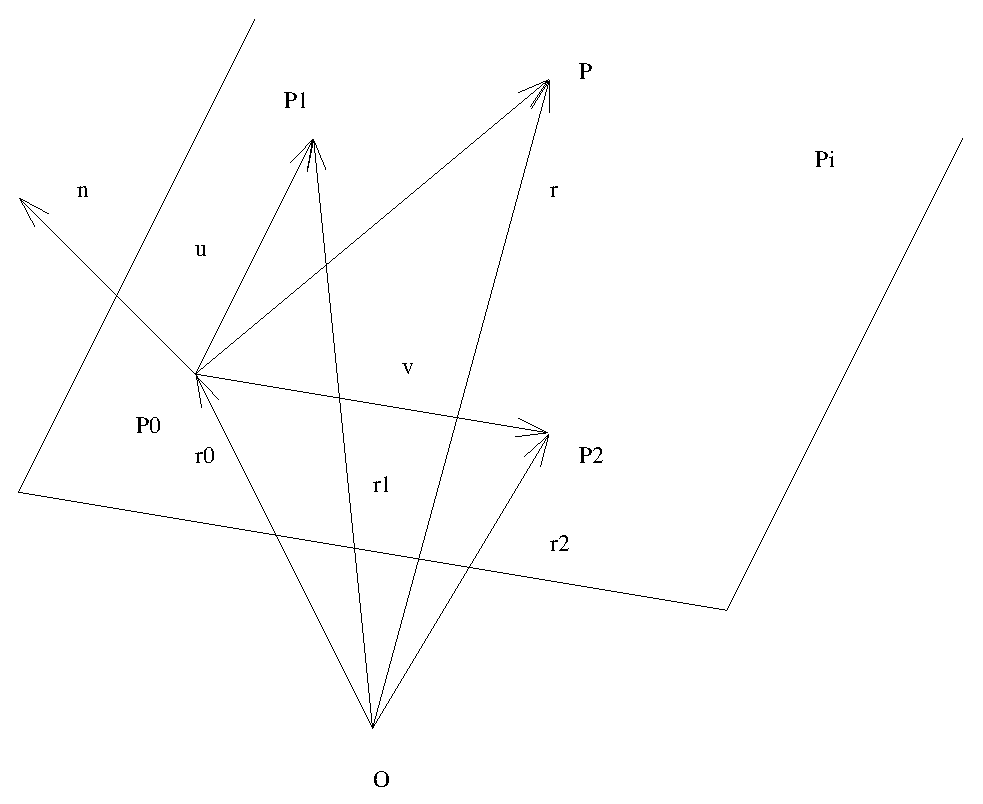
\includegraphics[height=1.5in]{../../modules/vectors/pictures/ok-plane_three_points.eps}
\column{0.6\textwidth}
\begin{itemize}
\item Given: three non-collinear points $P_0(\fcv{r}_0)$, $P_1(\fcv{r}_1)$, $P_2(\fcv{r}_2)$.
\item Goal: find equations fo plane $\mathcal{P}$ passing through $P_0$, $P_1$, and $P_2$.
\end{itemize}
\end{columns}
\only<2>{
The plane is parallel to $\fcv{u} = \fcv{P}_0\fcv{P}_1 = \fcv{r}_1 -\fcv{r}_0$ and passing through $P_0$ $\Rightarrow$ this problem was solved previously.

Normal $\fcv{n} = \fcv{u} \times \fcv{v} =
(\fcv{r}_1-\fcv{r}_0) \times (\fcv{r}_2-\fcv{r}_0)$  \\

\alert<1->{Implicit vectorial equation}:
  $$(\fcv{r}-\fcv{r}_0) \cdot \fcv{n} = 0$$
  %
  $$\boxed{(\fcv{r}-\fcv{r}_0) \cdot [(\fcv{r}_1-\fcv{r}_0) \times (\fcv{r}_2-\fcv{r}_0)] = 0}$$
%
$$\text{Vol}(R(\fcv{P}_0\fcv{P}, \fcv{P}_0\fcv{P}_1, \fcv{P}_0\fcv{P}_2)) = 0$$
  }

 \only<3>{
 \alert<1->{Implicit vectorial equation}: $(\fcv{r}-\fcv{r}_0) \cdot [(\fcv{r}_1-\fcv{r}_0) \times (\fcv{r}_2-\fcv{r}_0)] = 0$

Let the points have coordinates $P_0(x_0,y_0,z_0)$, $P_1(x_1,y_1,z_1)$, $P_2(x_2,y_2,z_2)$. $P(x,y,z)$ is on plane $\mathcal{P}$:\\

\alert<1->{Implicit scalar equation}:
%
$\left| \begin{array}{ccc}
          x-x_0 & y-y_0 & z-z_0 \\
          x_1-x_0 & y_1-y_0 & z_1-z_0 \\
          x_2-x_0 & y_2-y_0 & z_2-z_0	
         \end{array}
\right| = 0\; .$
%
  }
\end{frame}

